
\markboth{CAPITOLO 2. ESERCIZI A.A. 2017-18}{CAPITOLO 2. ESERCIZI A.A. 2017-18}
\begin{flushleft}
	\textbf{Esercizio 2.1} \textit{Determinare analiticamente gli zeri del polinomio}\\
	\begin{center}
		$P(x) = x^3 - 4x^2 + 5x - 2$
	\end{center}
	\textit{e la loro molteplicit�. Dire perch� il metodo di bisezione � utilizzabile per approssimarne uno a partire dall'intervallo di confidenza $[a, b] = [0, 3]$. A quale zero di P potr� tendere la successione generata dal metodo di bisezione a partire da tale intervallo? Costruire una tabella in cui si riportano il numero di iterazioni e di valutazioni di P richieste per valori decrescenti della tolleranza} tolx.\\
	\medskip
	\textbf{Soluzione:} Prendiamo in considerazione il nostro polinomio e vediamo subito che un suo zero � 1, infatti:\\
	con $\hat{x} = 1:$
	\begin{center}
		$P(1) = 1^3 -4*1^2 +5*1 - 2 =$\\
		$= 1 - 4 + 5 - 2 = 0$
	\end{center}
	A questo punto controlliamo la sua molteplicit�:
	\begin{center}
		$P'(x) = 3x^2 - 8x + 5$\\
		$P'(1) = 3 - 8 + 5 = 0$\\
		\medskip
		$P''(x) = 6x - 8$\\
		$P''(1) = 6 - 8 = -2$
	\end{center}
	La molteplicit� � 2 poich� la derivata seconda � la prima derivata in ordine che non viene annullata.\\
	\medskip
	Un'altro suo zero � 2:\\
	con $\hat{x} = 2:$
	\begin{center}
		$P(2) = 8 - 16 + 10 - 2 = 0$
	\end{center}
	\begin{center}
		$P'(2) = 12 - 16 + 5 = 1$
	\end{center}
	In questo caso la molteplicit� � 1.\\
	\medskip
	Il metodo di bisezione � utilizzabile nell'intervallo di confidenza $[0, 3]$ in quanto $P(a)P(b)<0$, precisando che in tale intervallo P tender� a 2:\\
	\begin{center}
		$P(0) = 0 - 0 + 0 - 2 = -2$\\
		$P(3) = 27 - 36 + 15 - 2 = 4$\\
		$-2 * 4 < 0$\\
	\end{center}
	\newpage{}
	Di seguito i risultati dell'esecuzione del metodo di bisezione utilizzando come intervallo di confidenza $[0, 3]$:\\
	\begin{center}
		\begin{tabular}{|c|c|c|}
			\hline
			\multicolumn{3}{|c|}{$P(x) = x^3 - 4x^2 + 5x -2$, $\qquad I=\left[0,3\right]$}\tabularnewline
			\hline
			\multicolumn{3}{|c|}{$\tilde{x}{\ensuremath{\approx}}2.0$}\tabularnewline
			\hline
			$tol_{x}$ & Approssimazione & Iterazioni\tabularnewline
			\hline
			$10^{-1}$	& $\tilde{x} = 2.062500000000000$ &	$i = 3$\tabularnewline
			\hline
			$10^{-2}$ &	$\tilde{x} = 1.992187500000000$ & $i = 6$\tabularnewline
			\hline
			$10^{-3}$ &	$\tilde{x} = 2.000976562500000$ & $i = 9$\tabularnewline
			\hline
			$10^{-4}$ &	$\tilde{x} = 2.000061035156250$ & $i = 13$\tabularnewline
			\hline
			$10^{-5}$ &	$\tilde{x} = 1.999992370605469$ & $i = 16$\tabularnewline
			\hline
			$10^{-6}$ &	$\tilde{x} = 2.000000953674316$ & $i = 19$\tabularnewline
			\hline
			$10^{-7}$ &	$\tilde{x} = 2.000000059604645$ & $i = 23$\tabularnewline
			\hline
			$10^{-8}$ &	$\tilde{x} = 1.999999992549419$ & $i = 26$\tabularnewline
			\hline
			$10^{-9}$ &	$\tilde{x} = 2.000000000931323$ & $i = 29$\tabularnewline
			\hline
			$10^{-10}$ & $\tilde{x} = 2.000000000058208$ &	$i = 33$\tabularnewline
			\hline
			$10^{-11}$ & $\tilde{x} = 1.999999999992724$ &	$i = 36$\tabularnewline
			\hline
			$10^{-12}$ & $\tilde{x} = 2.000000000000909$ &	$i = 39$\tabularnewline
			\hline
			$10^{-13}$ & $\tilde{x} = 2.000000000000057$ &	$i = 43$\tabularnewline
			\hline
			$10^{-14}$ & $\tilde{x} = 1.999999999999993$ &	$i = 46$\tabularnewline
			\hline
			$10^{-15}$ & $\tilde{x} = 2.000000000000001$ &	$i = 49$\tabularnewline
			\hline
		\end{tabular}
	\end{center}
	Notiamo come dopo 49 iterazioni otteniamo il risultato con tolleranza pari a $10^{-15}$.\\
	\newpage
	\textbf{Esercizio 2.2} \textit{Completare la tabella precedente riportando anche il numero di iterazioni e di valutazioni di P richieste dal metodo di Newton, dal metodo delle corde e dal metodo delle secanti (con secondo termine della successione ottenuto con Newton) a partire dal punto $x_{0} = 3$. Commentare i risultati riportati in tabella. E' possibile utilizzare $x_{0} = 5/3$ come punto di innesco?}\\
	\textbf{Soluzione:}
	\begin{center}
		\begin{tabular}{|c|c|c|c|}
			\hline
			\multicolumn{4}{|c|}{$P(x) = x^3 - 4x^2 + 5x -2$, \qquad $x_{0} = 3$}\tabularnewline
			\hline
			\multicolumn{4}{|c|}{$\tilde{x}{\ensuremath{\approx}}2.0$}\tabularnewline
			\hline
			$tol_{x}$ & Newton & Corde & Secanti\tabularnewline
			\hline
			$10^{-1}$ & $\tilde{x} = 2.00435, i = 4$ & $x = 2.35938, i = 3$ & $x = 2.05016, i = 4$\tabularnewline
			\hline
			$10^{-2}$ & $\tilde{x} = 2.00004, i = 5$ & $x = 2.06432, i = 13$ & $x = 2.00099, i = 6$\tabularnewline
			\hline
			$10^{-3}$ & $\tilde{x} = 2.00000, i = 6$ & $x = 2.00767, i = 29$ & $x = 2.00002, i = 7$\tabularnewline
			\hline
			$10^{-4}$ & $\tilde{x} = 2.00000, i = 6$ & $x = 2.00078, i = 47$ & $x = 2.00000, i = 8$\tabularnewline
			\hline
			$10^{-5}$ & $\tilde{x} = 2.00000, i = 7$ & $x = 2.00007, i = 66$ & $x = 2.00000, i = 9$\tabularnewline
			\hline
			$10^{-6}$ & $\tilde{x} = 2.00000, i = 7$ & $x = 2.00001, i = 84$ & $x = 2.00000, i = 9$\tabularnewline
			\hline
			$10^{-7}$ & $\tilde{x} = 2.00000, i = 7$ & $x = 2.00000, i = 102$	& $x = 2.00000, i = 9$\tabularnewline
			\hline
			$10^{-8}$ & $\tilde{x} = 2.00000, i = 7$ & $x = 2.00000, i = 120$ & $x = 2.00000, i = 10$\tabularnewline
			\hline
			$10^{-9}$ & $\tilde{x} = 2.00000, i = 8$ & $x = 2.00000, i = 139$ & $x = 2.00000, i = 10$\tabularnewline
			\hline
			$10^{-10}$ & $\tilde{x} = 2.00000, i = 8$ & $x = 2.00000, i = 157$ & $x = 2.00000, i = 10$\tabularnewline
			\hline
			$10^{-11}$ & $\tilde{x} = 2.00000, i = 8$ & $x = 2.00000, i = 175$ & $x = 2.00000, i = 10$\tabularnewline
			\hline
			$10^{-12}$ & $\tilde{x} = 2.00000, i = 8$ & $x = 2.00000, i = 193$ & $x = 2.00000, i = 11$\tabularnewline
			\hline
			$10^{-13}$ & $\tilde{x} = 2.00000, i = 8$ & $x = 2.00000, i = 211$ & $x = 2.00000, i = 11$\tabularnewline
			\hline
			$10^{-14}$ & $\tilde{x} = 2.00000, i = 8$ & $x = 2.00000, i = 230$ & $x = 2.00000, i = 11$\tabularnewline
			\hline
			$10^{-15}$ & $\tilde{x} = 2.00000, i = 8$ & $x = 2.00000, i = 247$ & $x = 2.00000, i = 11$\tabularnewline
			\hline
		\end{tabular}
	\end{center}
	Possiamo notare come il metodo pi� efficiente � quello di Newton, mentre il metodo meno efficiente � quello delle corde.\\
	No non � possibile utilizzare $x_{0} = 5/3$ come punto di innesco in quanto $5/3$ � uno zero della derivata prima.\\
	\medskip
	\newpage
	\textbf{Esercizio 2.3} \textit{Costruire una seconda tabella analoga alla precedente relativa ai metodi di Newton, di Newton modificato e di accelerazione di Aitken applicati alla funzione polinomiale P a partire dal punto di innesco $x_{0} = 0$. Commentare i risultati riportati in tabella.}\\
	\medskip
	\textbf{Soluzione:}
	Avendo valutato precedentemente che la molteplicit� di P � 2 applichiamo il metodo di Newton modificaton con coefficente del termine di correzione $m = 2$:
	\begin{center}
		\begin{tabular}{|c|c|c|c|}
			\hline
			\multicolumn{4}{|c|}{$P(x) = x^3 - 4x^2 + 5x -2$, \qquad $x_{0} = 0$}\tabularnewline
			\hline
			\multicolumn{4}{|c|}{$\tilde{x}{\ensuremath{\approx}}1.0$}\tabularnewline
			\hline
			$tol_{x}$ & Newton & Newton modificato & Aitken\tabularnewline
			\hline
			$10^{-1}$ & $\tilde{x} = 0.89599, i = 4$ & $x = 0.99607, i = 3$ & $x = 1.00056, i = 3$\tabularnewline
			\hline
			$10^{-2}$ & $\tilde{x} = 0.99289, i = 8$ & $x = 0.99999, i = 4$ & $x = 1.00000, i = 4$\tabularnewline
			\hline
			$10^{-3}$ & $\tilde{x} = 0.99911, i = 11$ & $x = 1.00000, i = 5$ & $x = 1.00000, i = 4$\tabularnewline
			\hline
			$10^{-4}$ & $\tilde{x} = 0.99994, i = 15$ & $x = 1.00000, i = 5$ & $x = 1.00000, i = 5$\tabularnewline
			\hline
			$10^{-5}$ & $\tilde{x} = 0.99999, i = 18$ & $x = 1.00000, i = 5$ & $x = 1.00000, i = 5$\tabularnewline
			\hline
			$10^{-6}$ & $\tilde{x} = 1.00000, i = 21$ & $x = 1.00000, i = 6$ & $x = 1.00000, i = 5$\tabularnewline
			\hline
			$10^{-7}$ & $\tilde{x} = 1.00000, i = 25$ & $x = 1.00000, i = 6$	& $x = 1.00000, i = 5$\tabularnewline
			\hline
			$10^{-8}$ & $\tilde{x} = 1.00000, i = 29$ & $x = 1.00000, i = 6$ & $x = 1.00000, i = 6$\tabularnewline
			\hline
			$10^{-9}$ & $\tilde{x} = 1.00000, i = 29$ & $x = 1.00000, i = 6$ & $x = 1.00000, i = 6$\tabularnewline
			\hline
			$10^{-10}$ & $\tilde{x} = 1.00000, i = 29$ & $x = 1.00000, i = 6$ & $x = 1.00000, i = 6$\tabularnewline
			\hline
			$10^{-11}$ & $\tilde{x} = 1.00000, i = 29$ & $x = 1.00000, i = 6$ & $x = 1.00000, i = 6$\tabularnewline
			\hline
			$10^{-12}$ & $\tilde{x} = 1.00000, i = 29$ & $x = 1.00000, i = 6$ & $x = 1.00000, i = 6$\tabularnewline
			\hline
			$10^{-13}$ & $\tilde{x} = 1.00000, i = 29$ & $x = 1.00000, i = 6$ & $x = 1.00000, i = 6$\tabularnewline
			\hline
			$10^{-14}$ & $\tilde{x} = 1.00000, i = 29$ & $x = 1.00000, i = 6$ & $x = 1.00000, i = 6$\tabularnewline
			\hline
			$10^{-15}$ & $\tilde{x} = 1.00000, i = 29$ & $x = 1.00000, i = 6$ & \tabularnewline
			\hline
		\end{tabular}
	\end{center}
	Come era prevedibile notiamo che il metodo di Newton converge linearmente. Il metodo di Newton modificato e quello di Aitken performano similmente e notiamo che il costo di discosta di poco.\\
\newpage
\textbf{Esercizio 2.4} \textit{Definire una procedura iterativa basata sul metodo di Newton per approssimare \(\sqrt\alpha \), per un assegnato \(\alpha > 0\). Costruire una tabella dove si riportano le successive approssimazioni ottenute e i corrispondenti errori assoluti (usare l'approssimazione di Matlab di \(\sqrt\alpha \) per il calcolo dell'errore) nel caso in cui \(\alpha=5\) partendo da \(x_0=5\).}\\
\textbf{Soluzione:}
Il seguente metodo produrr� la tabella richiesta:
\lstinputlisting[language=Matlab]{Capitolo2/es2_4.m}
\begin{center}
	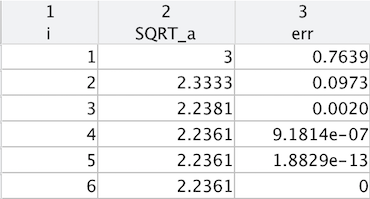
\includegraphics[scale=1]{Capitolo2/es2_4.png}
\end{center}
\newpage
\textbf{Esercizio 2.5} \textit{
Definire una procedura iterativa basata sul metodo delle secanti sempre per approssimare \(\sqrt\alpha \), per un assegnato \(\alpha > 0\). Completare la tabella precedente aggiungendovi i risultati ottenuti con tale precedura partendo da \(x_0=5\) e \(x_1=3\). Commentare i risultati riportati in tabella.}\\
\textbf{Soluzione:}
\lstinputlisting[language=Matlab]{Capitolo2/es2_5.m}
\begin{center}
	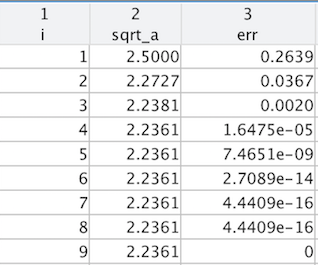
\includegraphics[scale=1]{Capitolo2/es2_5.png}
\end{center}
Dal risultato ottenuto possiamo notare come a differenza del metodo di newton il metodo delle secanti converge \(\sqrt\alpha \) meglio nelle prime iterazioni, ma il metodo di Newton converge poi con pi� precisione convergendo pi� velocemente verso il risultato esatto.\\
\newpage
\end{flushleft}
